\documentclass[compress,12pt]{beamer}
\usepackage{caption}
\usepackage{subcaption}
\usetheme{Arguelles}
\usepackage{color}
\usepackage{tcolorbox}
\usepackage{xcolor}
\usepackage{booktabs}
\usepackage{algorithm,algpseudocode}
\usepackage{amsfonts, amsmath, amssymb}
\newcommand{\myRed}[1]{\textcolor{red}{#1}}

\title{MATH 512 - Project 3}
\subtitle{}
\event{}
\date{}
\author{Wasif Ahmed, Haoxiang Deng, Jacob Fein-Ashley, Kanav Malhotra, Longzhe Yang}


\begin{document}

\frame[plain]{\titlepage}

\section{Question 1}


\begin{frame}{Question 1}

    \begin{itemize}
        \item We wish to estimate the following expectation $\mathbb{E}[W_3^2 + \sin(W_3) + 2\exp{W_3}]$, where $W_t$ is a standard Wiener process.

        \item We draw 200,000 pseudo-random samples in the range $[0, \sqrt{3}]$, with each entry as an element $\in W$ ($W$ is a vector).

        \item Scale $W_3^2 + \sin(W_3) + 2\exp{W_3}$ and we take the sample mean, yielding $\boxed{11.97068421176774}$.

    \end{itemize}
 
\end{frame}

\begin{frame}{Question 1 Continued}
    We plot the expected value of the function as it varies with the number of samples in Figure~\ref{fig:convergence}.

    \begin{figure}
        \centering
        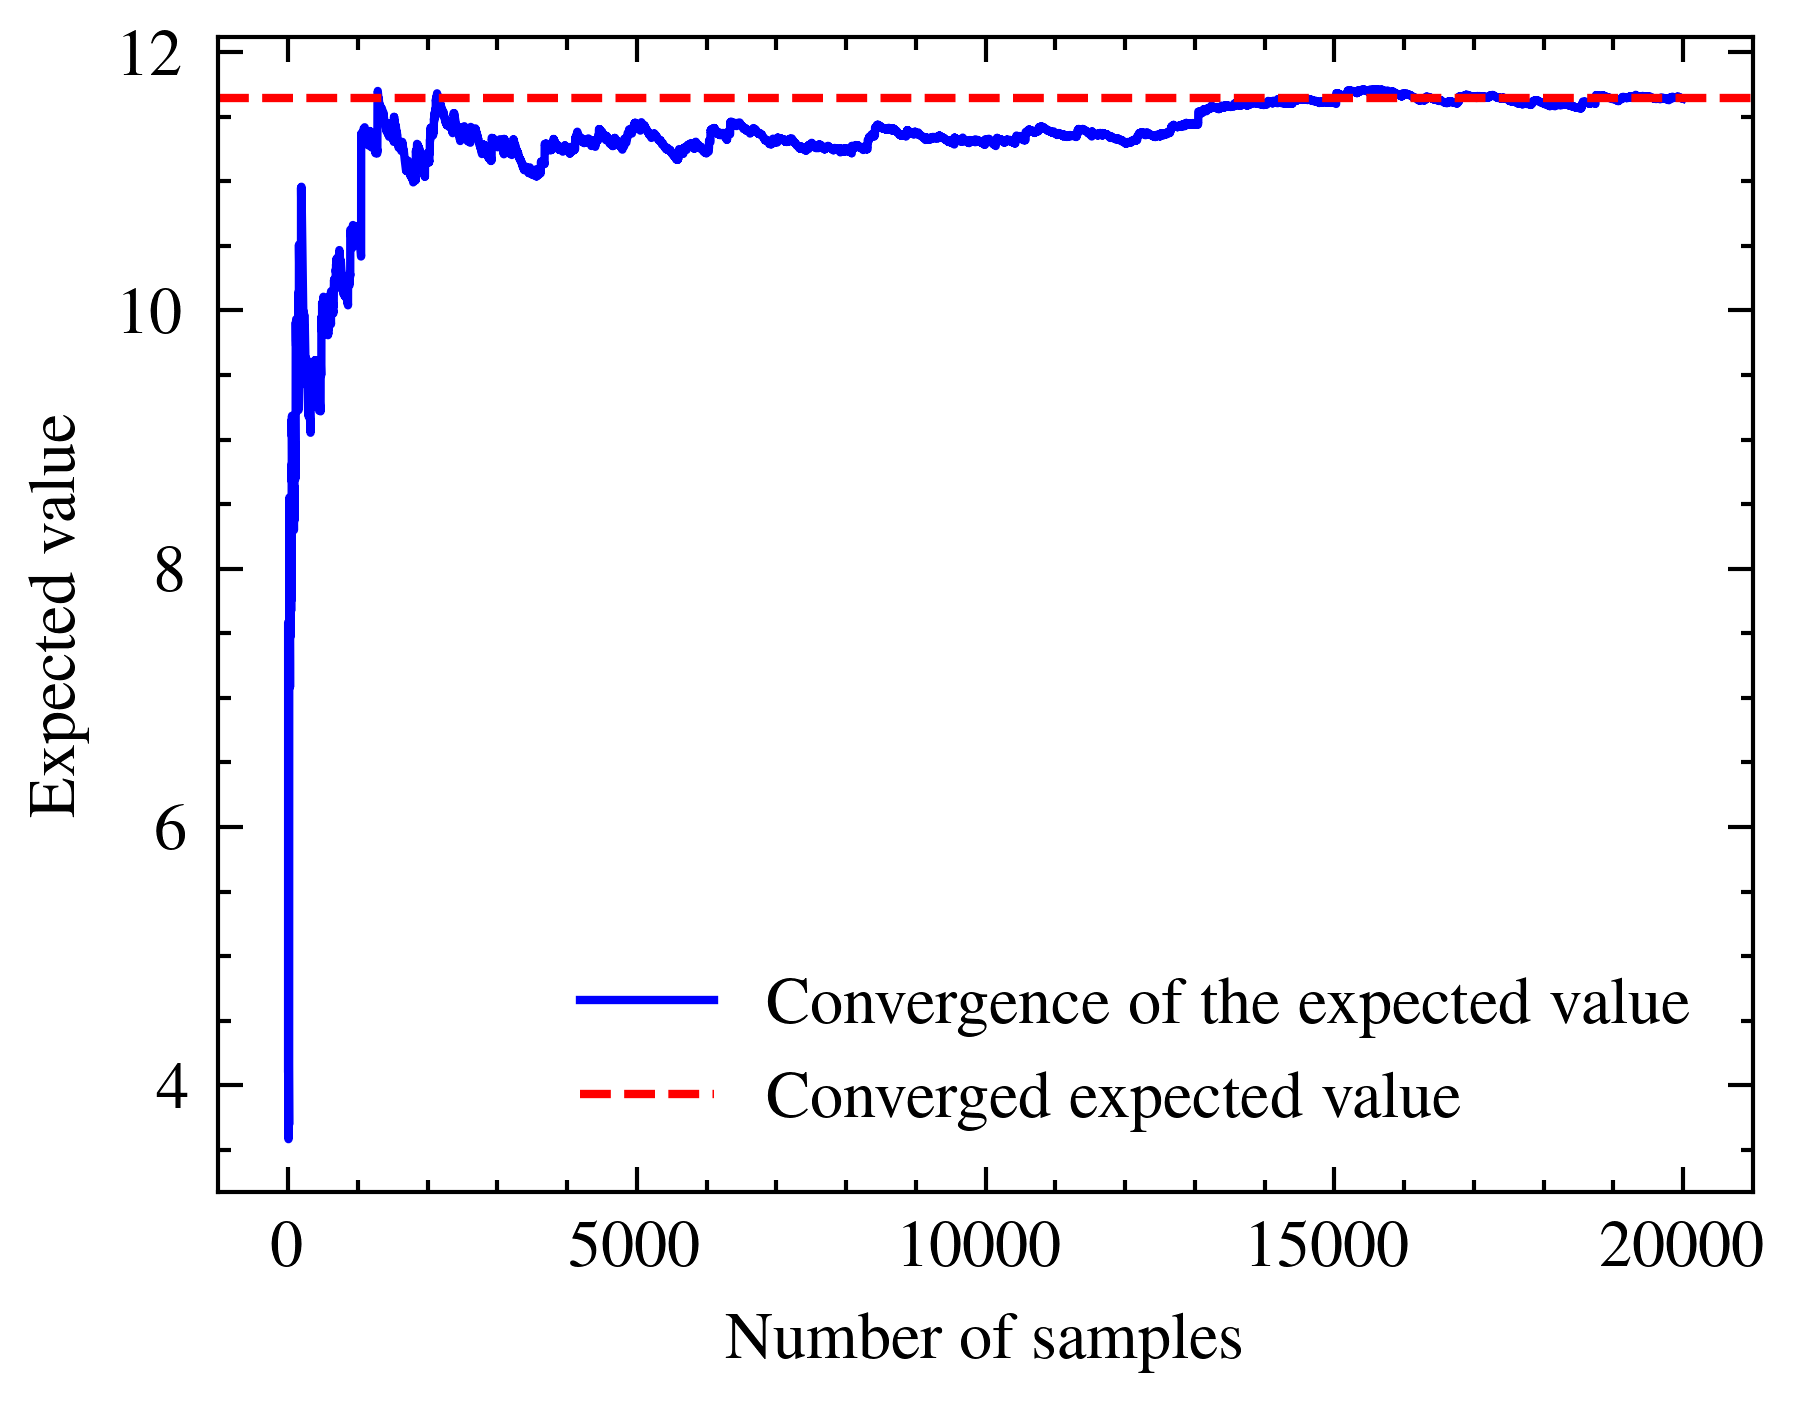
\includegraphics{imgs/convergence.png}
        \caption{Convergence of the Given Expectation Over 200,000 Iterations}
        \label{fig:convergence}
    \end{figure}
\end{frame}

\begin{frame}{Question 1 Continued}
    Additionally, we plot a histogram for the function below.

    \begin{figure}
        \centering
        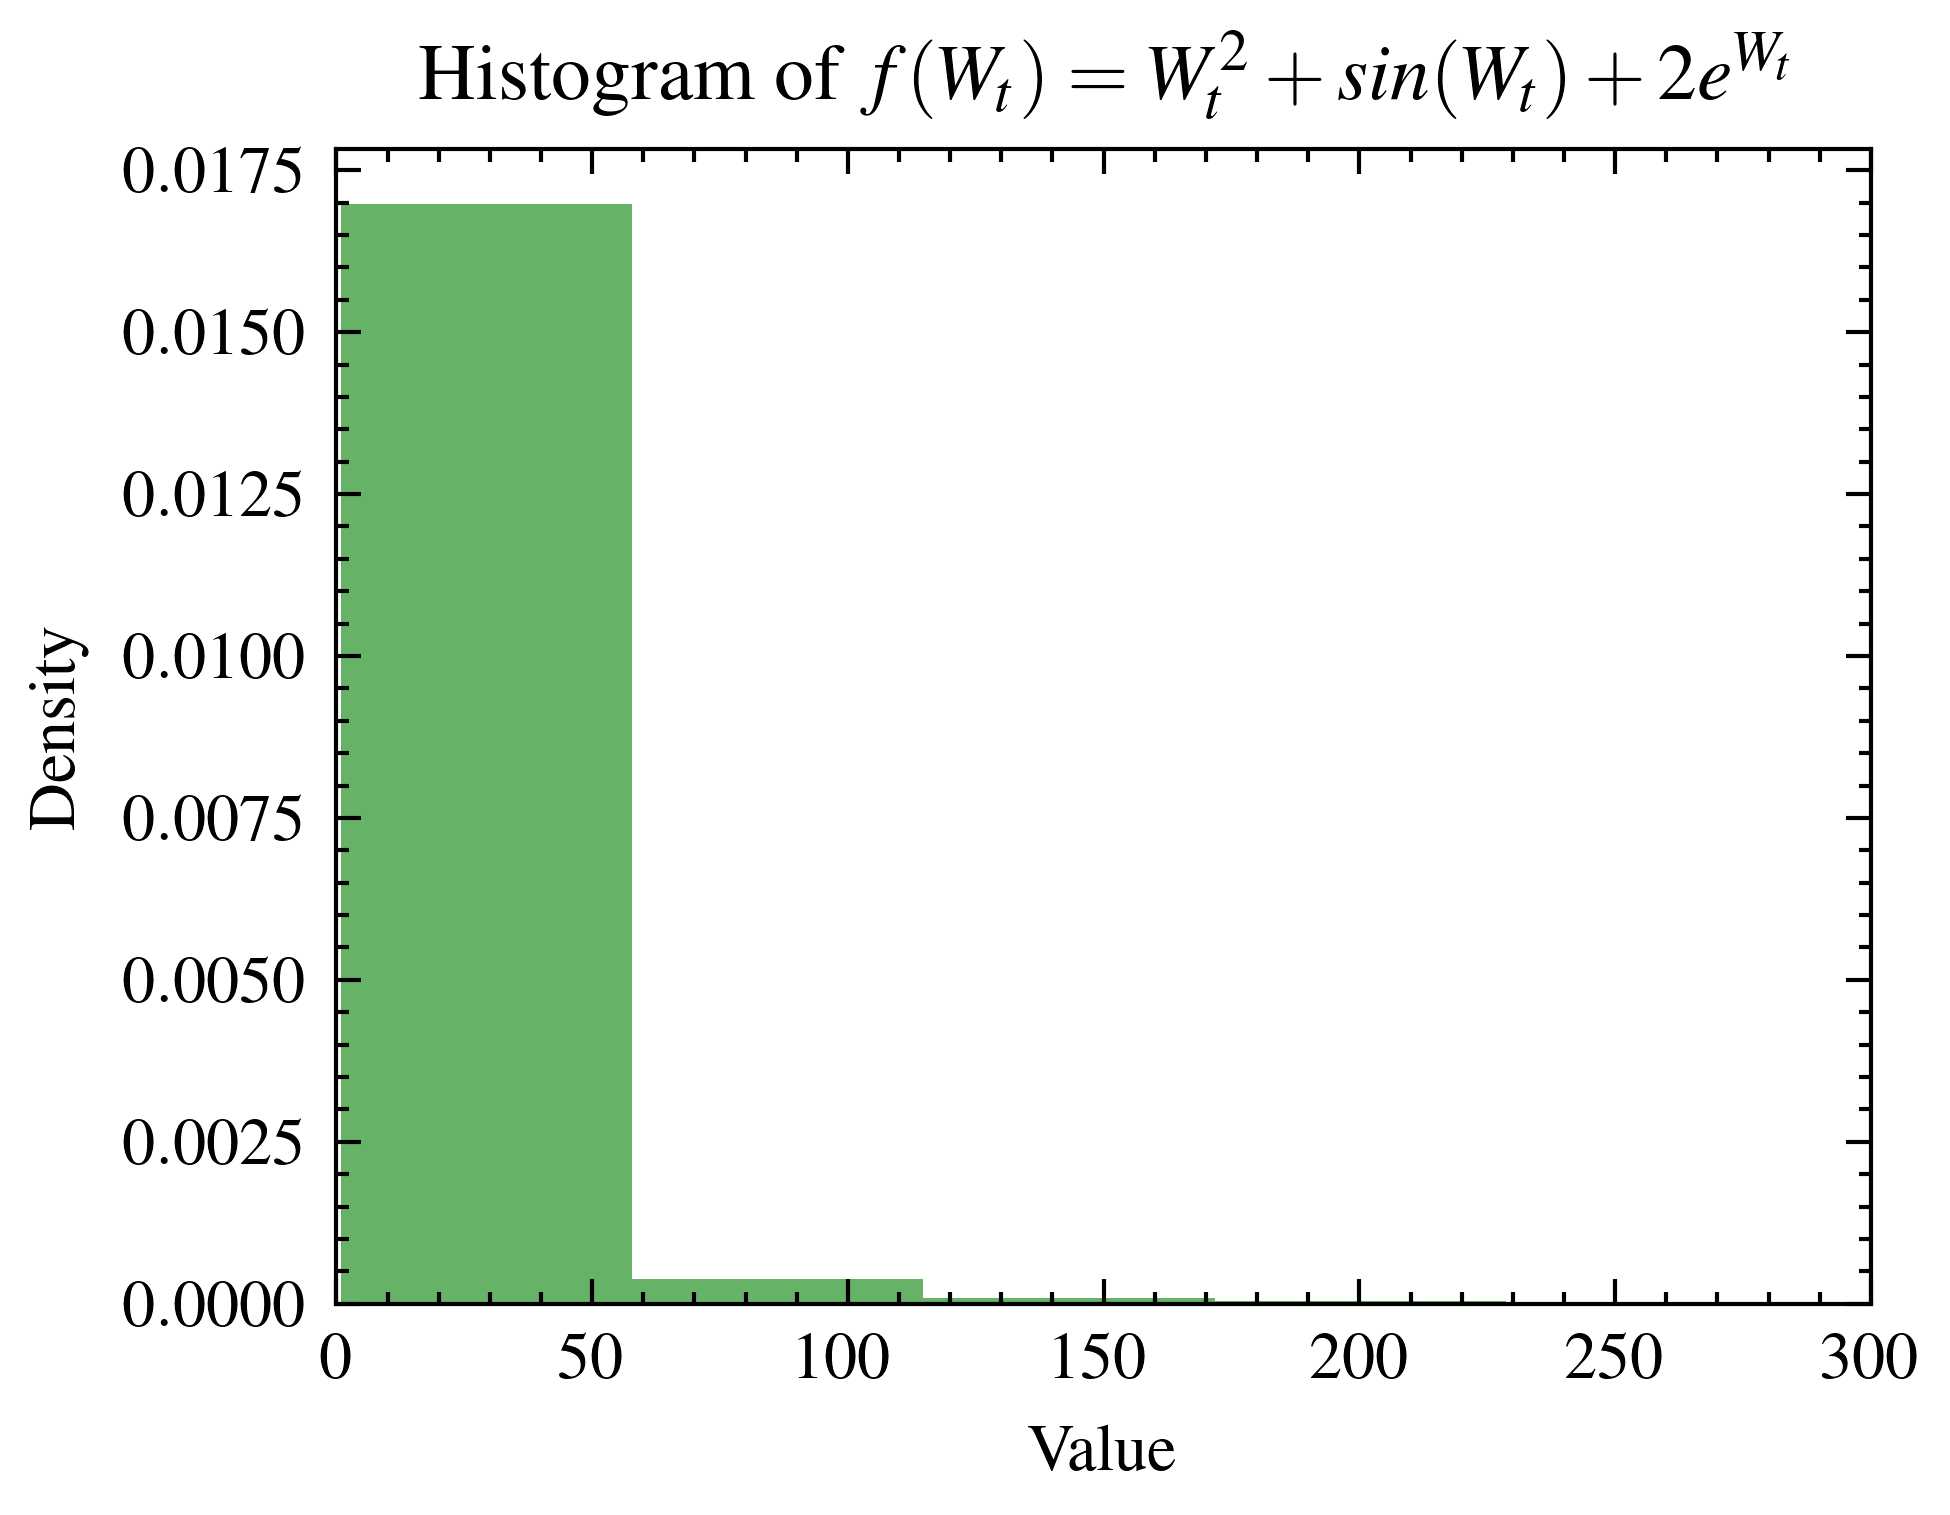
\includegraphics{imgs/histogram.png}
        \caption{Histogram of the Function}
        \label{fig:convergence}
    \end{figure}
\end{frame}

\begin{frame}{Question 1 Continued}
    Although there is a large density of values close to the value $0$, we find a variance of the function of $1661.25$! We find the contributing variable that explains the most variance in the following way:
    % Mean of W_t^2 = 2.97729902284579
% Variance of W_t^2 = 17.592746124707148
% Mean of sin(W_t) = -0.0018507484598128696
% Variance of sin(W_t) = 0.49848579671005355
% Mean of 2e^W_t = 8.85261926148378
% Variance of 2e^W_t = 1481.7866965481849
    \begin{table}[H]
        \centering
        \begin{tabular}{@{}lll@{}}
        \toprule
        Variable & Mean & Variance \\ \midrule
        $W_t^2$ & 2.97729902284579 & 17.592746124707148 \\
        $\sin(W_t)$ & -0.0018507484598128696 & 0.49848579671005355 \\
        $2e^{W_t}$ & 8.85261926148378 & 1481.7866965481849 \\ \bottomrule
        \end{tabular}
    \end{table}

    Thus, $2e^{W_t}$ contributes the most to the variance of the function with an extremely large variance.
\end{frame}


\begin{frame}{Question 2}
    With $S_t$ as a Geometric Brownian Motion process, we have $S_t = S_0e^{(\sigma W_t + (r - \frac{\sigma^2}{2})t)}$ where $r = 0.05$, $\sigma = 0.20$, $S_0 = 90$, and $W_t$ is a standard Wiener process. We wish to estimate $\mathbb{E}[S_3]$.
\end{frame}

\begin{frame}{Question 2 Continued}

    \begin{itemize}
        \item We use a sufficiently large simulation size (20,000) to simulate $\mathbb{E}[S_3]$. The Wiener process is simulated using NumPy's
        built-in random number generator in the range $[0, \sqrt{t}]$, with $t = 3$.
        \item We note that $B_t$ is a GBM, i.e. $B_t$ has moment generating function $\mathbb{E}[e^{uB_t}] = e^{\frac{u^2}{2}t} (1)$
        \item So using (1) with $u=\sigma$ we calculate our expected $\mathbb{E}[S_t] = S_0e^{({r-\frac{\sigma^2}{2}t})}e^{(\frac{\sigma^2}{2}t)} = S_0e^{rt}$
    
    \end{itemize}

    \begin{tcolorbox}
        Simulated $\mathbb{E}[S_3]$ is $\boxed{104.2625934286796}$\\
        Expected $\mathbb{E}[S_3]$ is $\boxed{104.56508184554548}$
    \end{tcolorbox}
\end{frame}


\begin{frame}{Question 3}

    Our goal is to evaluate the following expected value and probability:
    \begin{itemize}
        \item $\mathbb{E}(X^{0.6}_{2})$
        \item $\mathbb{P}(X^{0.6}> 2)$
    \end{itemize}

    The Ito's processes $X$ evolve according to the following SDE:
    \begin{equation*}
        dX_t = \left( \frac{1}{4} + \frac{1}{3}X_t \right) dt + \frac{3}{5} dW_t, \quad X_0 = 2
    \end{equation*}
    where $W$ is a standard Wiener process.

\end{frame}


\begin{frame}{Question 3 Continued}
    \begin{itemize}
        \item This is an Ornstein-Uhlenbeck problem with a drift.
        $$dX_t=\theta (\mu -X_t)dt+\sigma dW_t$$
        \item The general solution can be written as:
        $$X_t=X_0e^{-\theta t}+\mu (1-e^{-\theta t})+\sigma \int_0^t e^{-\theta(t-s)}dW_s$$
        \item The expectation value can be calculated as,
        $$E[X_t]=X_0e^{-\theta t}+\mu (1-e^{-\theta t})$$
    \end{itemize}
    
  %  \begin{algorithmic}
   %     \For{$i = 1, 2, \ldots, N$}
    %        \State $dW = \sqrt{dt} Z_i$
    %        \State $X_{t_i} = X_{t_{i-1}} + \left( \frac{1}{4} + %\frac{1}{3}X_{t_{i-1}} \right) dt + \frac{3}{5} dW$
    %        \State Update $W_{t_i} = W_{t_{i-1}} + dW$
    %    \EndFor
    %\end{algorithmic}
\end{frame}

\begin{frame}{Question 3 Continued}
    \begin{itemize}
        \item In our case, the solution can be written as,
        $$X_t=-\frac{3}{4}+\frac{5}{4}e^{\frac{t}{3}}+\frac{3}{5}\int_0^t e^{\frac{1}{3}(t-s)}dW_s.$$
        \item The stochastic part is, $$N(0,\sqrt{\frac{3}{2}(-1+e^{\frac{2t}{5}})}).$$
        \item The expectation value is,
        $$E[X_t]=-\frac{3}{4}+\frac{5}{4}e^{\frac{t}{3}}$$.
    \end{itemize}
    

\end{frame}


\begin{frame}{Question 3 Continued}
    \begin{figure}
        \centering
        \includegraphics[scale=0.25]{imgs/stochastic_plot.jpeg}
        \caption{$X_t$ as a function of time}
        % \label{fig:probability}
    \end{figure}

\end{frame}

\begin{frame}{Question 3 Continued}
    \begin{itemize}
        \item data = RandomVariate[NormalDistribution[0, Sqrt[3/2 (-1 + Exp[4/5])]],$10^4$];
        Mean[data]=0.0047327
        \item N[-3/4 + 5/4 Exp[2/3]]=1.68467
        

    \end{itemize}
    
  %  \begin{algorithmic}
   %     \For{$i = 1, 2, \ldots, N$}
    %        \State $dW = \sqrt{dt} Z_i$
    %        \State $X_{t_i} = X_{t_{i-1}} + \left( \frac{1}{4} + %\frac{1}{3}X_{t_{i-1}} \right) dt + \frac{3}{5} dW$
    %        \State Update $W_{t_i} = W_{t_{i-1}} + dW$
    %    \EndFor
    %\end{algorithmic}
\end{frame}




\begin{frame}{Question 4}
    We consider the following SDE:
    \begin{equation*}
        dX_t = aX_t dt + bX_t dW_t, \quad X_0 = 100, \quad a = 0.07, \quad b = 0.12
    \end{equation*}

    \begin{itemize}
        \item We simulate this stochastic process using the discretization schemes of Euler-Maruyama.
        \item We compare the simulation with the analytical solution.
    \end{itemize}

    We use the following algorithm to simulate the process:
     
    \begin{algorithmic}
        \For{$i = 1, 2, \ldots, N$}
            \State $dW = \sqrt{dt} Z_i$
            \State $X_{t_i} = X_{t_{i-1}} + aX_{t_{i-1}} dt + bX_{t_{i-1}} dW$
            \State Update $W_{t_i} = W_{t_{i-1}} + dW$
        \EndFor
    \end{algorithmic}

    With the analytical solution given by $X_{\text{analytical}} = X_0 \exp((a - b^2/2)t + bW)$.
\end{frame}

\begin{frame}{Question 4 Continued}
    \begin{figure}
        \centering
        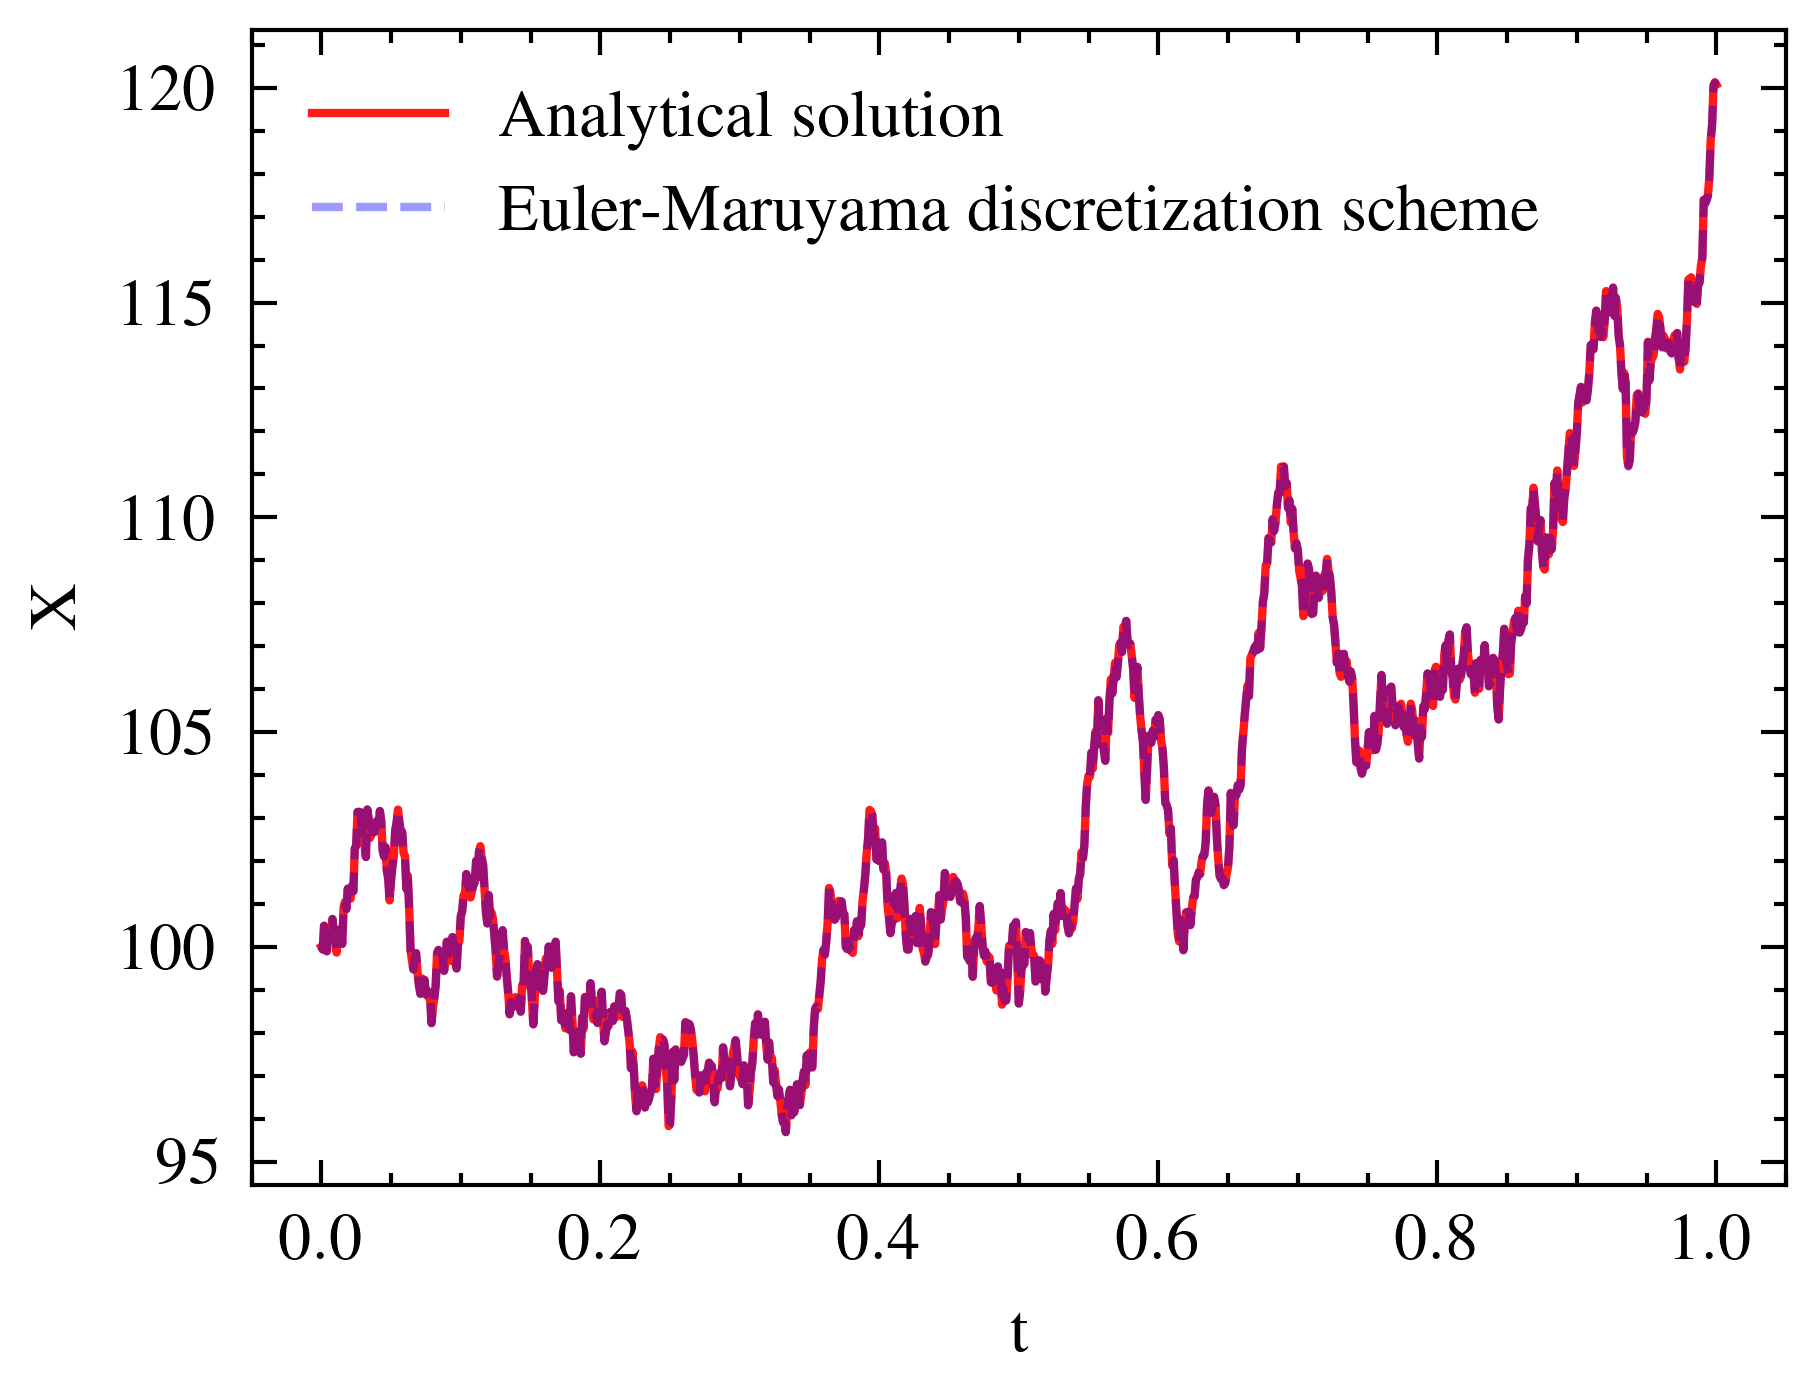
\includegraphics{imgs/eulermaruyama.png}
        \caption{Comparison of the Analytical Solution and the Euler-Maruyama Method}
        % \label{fig:question4}
    \end{figure}
\end{frame}

\begin{frame}{Question 4 Continued}
    We get a very close match between the analytical solution and the Euler-Maruyama method. The Euler-Maruyama method is a good approximation for the analytical solution. We calculate
    the sum of the absolute difference between the two methods and find that the average percent difference
    \begin{equation*}
        \text{Average Percent Difference} = \frac{1}{N} \sum_{i=1}^{N} \left| \frac{X_{\text{analytical}} - X_{\text{Euler-Maruyama}}}{X_{\text{analytical}}} \right|
    \end{equation*}
    is $\approx 0.01365803539\%$ and varies with the function.
\end{frame}

\begin{frame}{Question 4 Continued}
    \begin{figure}
        \centering
        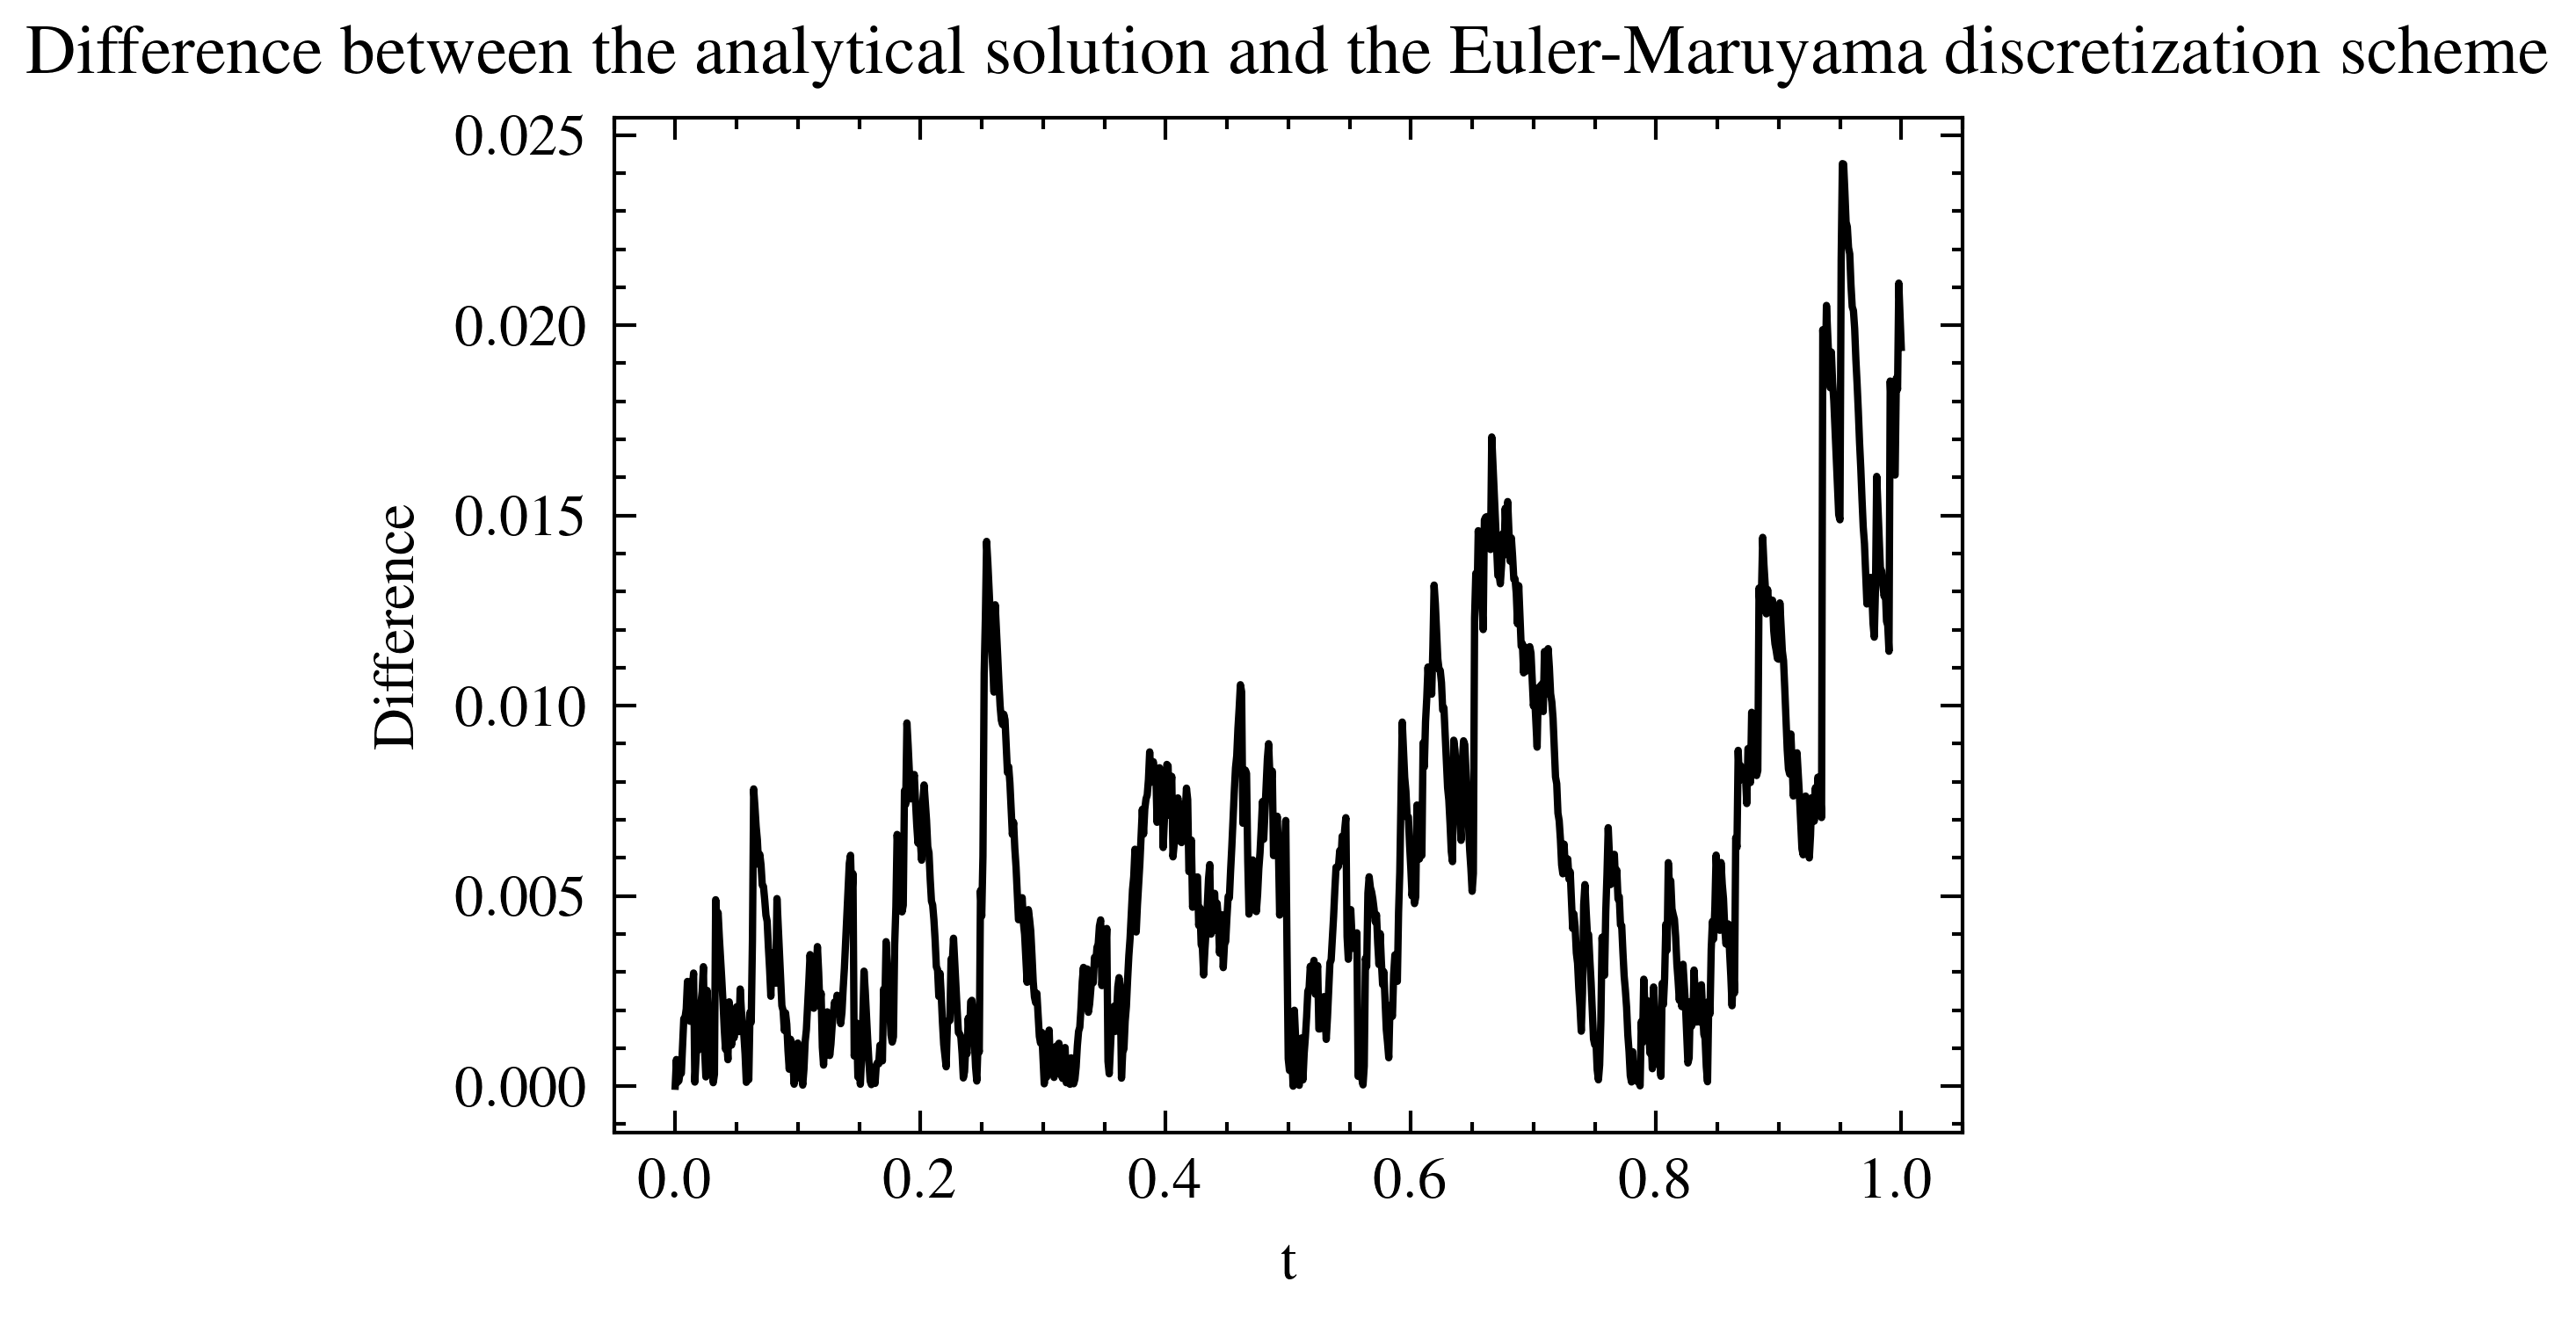
\includegraphics{imgs/difference.png}
        \caption{Difference Between the Analytical Solution and the Euler-Maruyama Method}
        % \label{fig:question4}
    \end{figure}
\end{frame}

\End
\begin{frame}[plain,standout]
      \centering
      Questions?
\end{frame}

\end{document}
